\chapter{Conclusiones y Recomendaciones}

\section{Nomenclatura}
Para el correcto análisis de la información referida, primeramente se han de
explicar algunos términos a ser utilizados:

\begin{description}
\item [Usuario] Persona que tiene el potencial de utilizar el sistema, cosa que
no implica que lo use.
\item [Rol] Definición del conjunto de funciones del sistema, disponibles para
los usuarios.
\item [Docente] Tipo de rol definido en el sistema, y que tiene la intención de
representar a un profesor.
\item [Espacio virtual] Lugar del sistema donde los usuarios pueden compartir
recursos.
\item [Materia] Tipo de espacio virtual de tipo formal, que engloba una
tópico determinado y que puede contener uno o varios grupos.
\item [Grupo] Tipo de espacio virtual de tipo formal, que es regida por un
docente y que define una forma de enseñanza independiente de otros espacios
virtuales.
\item [Recurso] Pieza de información creada por los usuarios, que es compartida
a todos los usuarios de un espacio virtual determinado.
\item [Actividad] Indicador del sistema que mide el numero de recursos creados
por un usuario.
\item [Participación] Indicador del sistema que mide el numero de comentarios
creados por un usuario.
\item [Contactos] Usuarios del sistema que poseen algún tipo de vinculo con
otro usuario.
\item [Enlace débil] Es el tipo de relación entre dos usuarios, en el que solo
uno de ellos reconoce al otro.
\item [Enlace fuerte] Es el tipo de relación entre dos usuarios, en el que
ambos se reconocen.
\item [Sociabilidad] Indicador del sistema que mide el numero de enlaces, ya
sean fuertes o débiles, que posee un usuario.
\item [Popularidad] Indicador del sistema que mide el grado de valoración de
los usuarios hacia los recursos de un usuario.
\item [Audiencia] Es el conjunto de usuarios que únicamente vieron el recurso,
sin realizar otra acción hacia este.
\item [Calificadores] Es el conjunto de usuarios que mostraron un interés
explicito hacia un recurso en particular.
\end{description}

%Las relaciones existentes entre los elementos del sistema son resumidos en la
%Figura \ref{nomenclatura}.
%\begin{figure}[H]
%\centering
%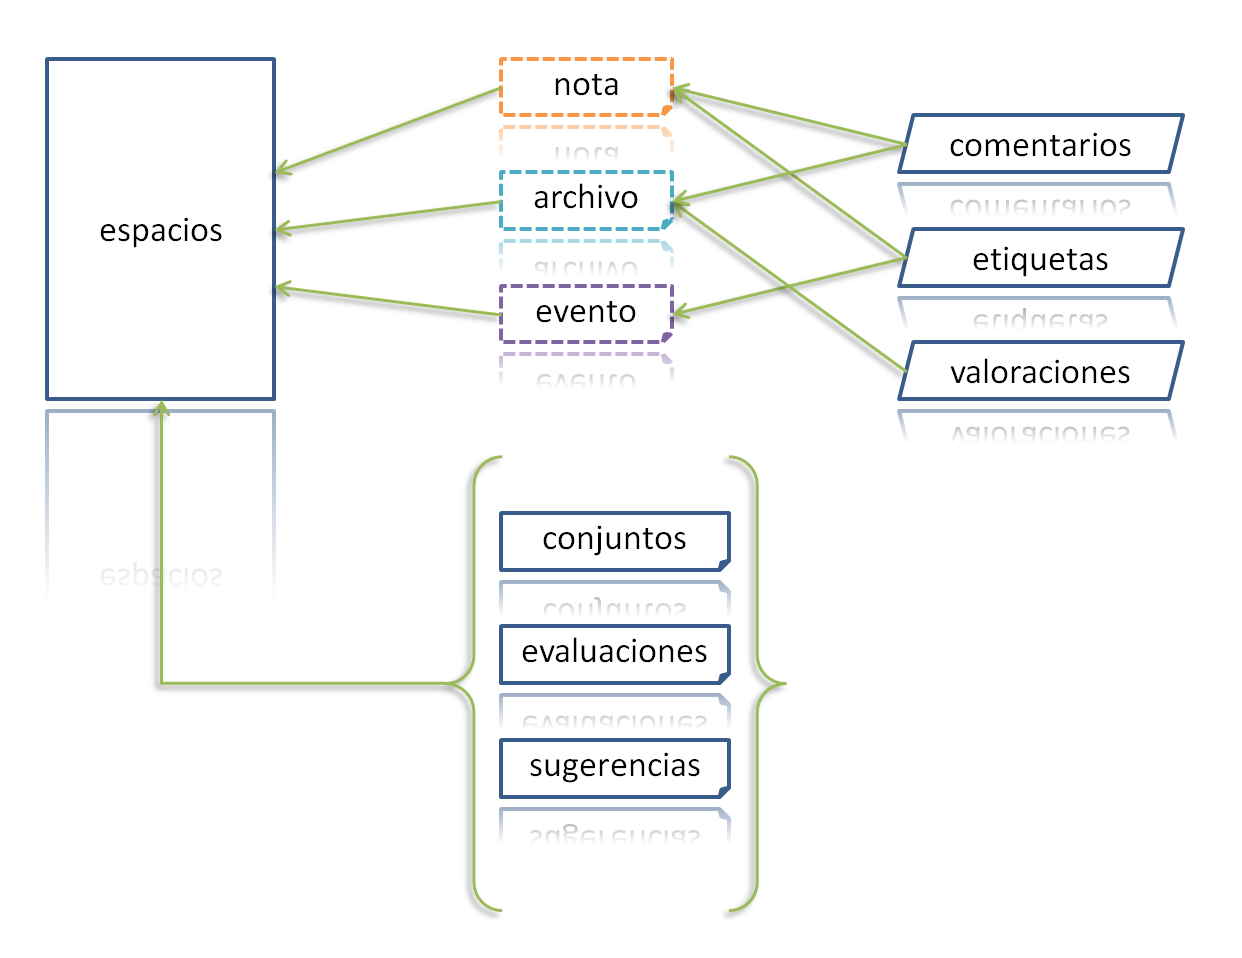
\includegraphics[scale=0.25]{graphics/nomenclatura.png}
%\caption {Relaci\'on entre los conceptos utilizados en el sistema}
%\label {nomenclatura}
%\end{figure}

\section{Resultados}
Definidos los términos a utilizarse, a continuación se presentan los resultados
generados:

\subsection{Contexto}
\begin{center}
\begin{tabular}{|l|l|}
\hline
Sitio web & yachay.memi.umss.edu.bo \\
Periodo académico & I/2011 \\
Tiempo de evaluación: & 325 días. \\
Fecha de inicio: & 23 de Septiembre del 2010. \\
Fecha de fin: & 14 de Agosto del 2011. \\
Lugar de evaluación: & Carrera de Informática y Sistemas (UMSS). \\
Caídas del servidor: & 4. \\
Tiempo del servidor fuera de linea: & 2 semanas acumuladas. \\
Docentes participantes: & 4. \\
Materias participantes: & 4. \\
Grupos participantes: & 8. \\
Usuarios participantes: & 542 (estudiantes de primeros semestres). \\
Espacios virtuales creados: & 33. \\
Recursos publicados: & 68. \\
\hline
\end{tabular}
\end{center}

\subsection{Usuarios}

%En términos de uso, puede apreciarse en la Figura \ref{usuarios_tabla_1} las
%diferentes formas de comportamiento de los usuarios, según el rol que
%desempeñan en el sistema.
%Destaca en esta tabla la disparidad entre el rol de estudiante y los demás
%roles, como puede verse en la Figura \ref{usuarios_bars_1}, del conjunto de
%usuarios registrados, únicamente el 20\% ingreso alguna vez al sistema,
%Es de rescatar además, que los usuarios fueron registrados automáticamente por
%sus respectivos docentes.

%\begin{figure}[H]
%\centering
%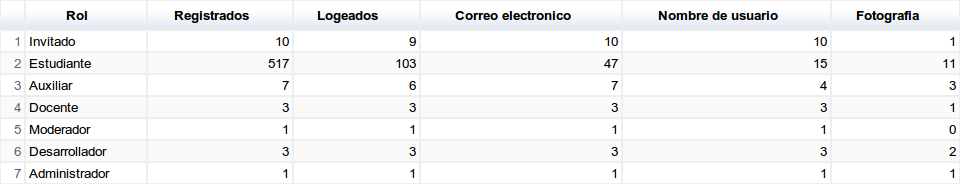
\includegraphics[scale=0.4]{graphics/usuarios_tabla_1.png}
%\caption {Intenci\'on de los usuarios clasificados por rol}
%\label {usuarios_tabla_1}
%\end{figure}

%\begin{figure}[H]
%\centering
%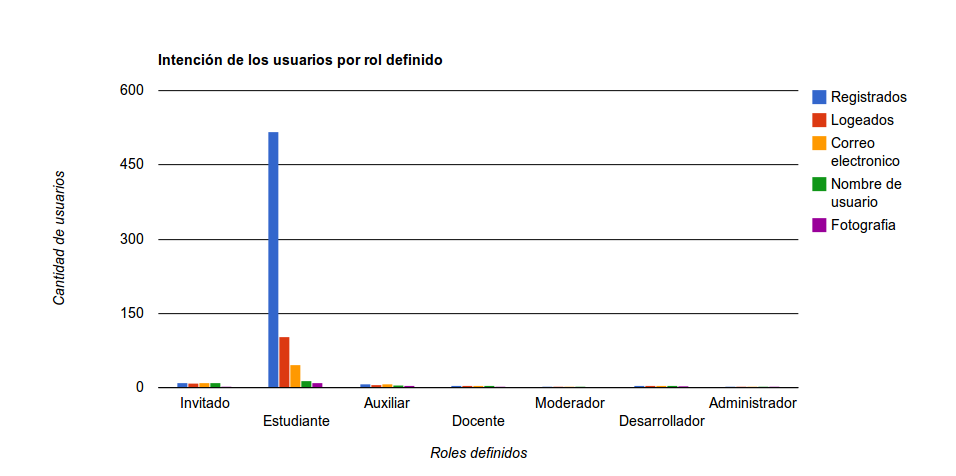
\includegraphics[scale=0.4]{graphics/usuarios_bars_1.png}
%\caption {Diagrama de barras de la intenci\'on de los usuarios clasificados
%por rol}
%\label {usuarios_bars_1}
%\end{figure}

%Puede verse en la Figura \ref{usuarios_pie_1} como el predominio en cantidad de
%los estudiantes va decayendo progresivamente en intención frente a los otros
%roles. Considerando los escasa cantidad de atractivos que posee el sistema es
%importante considerar una audiencia de 126 personas como el primer paso hacia
%la construcción de un lugar común para el estudio realizado.\\

%Respecto a la actividad de los usuarios sobre el sistema, puede verse en la
%Figura \ref{usuarios_tabla_2} la escasisima actividad, participación y
%popularidad en todos los roles, exceptuando el de los desarrolladores. Puede
%verse también en la Figura \ref{usuarios_bars_2} el prometedor indicador de
%sociabilidad, que como puede verse en la Figura \ref{usuarios_pie_2} es el mas
%homogéneo, lo que augura una conectividad mas que deseable para los usuarios.

%\begin{figure}[H]
%\centering
%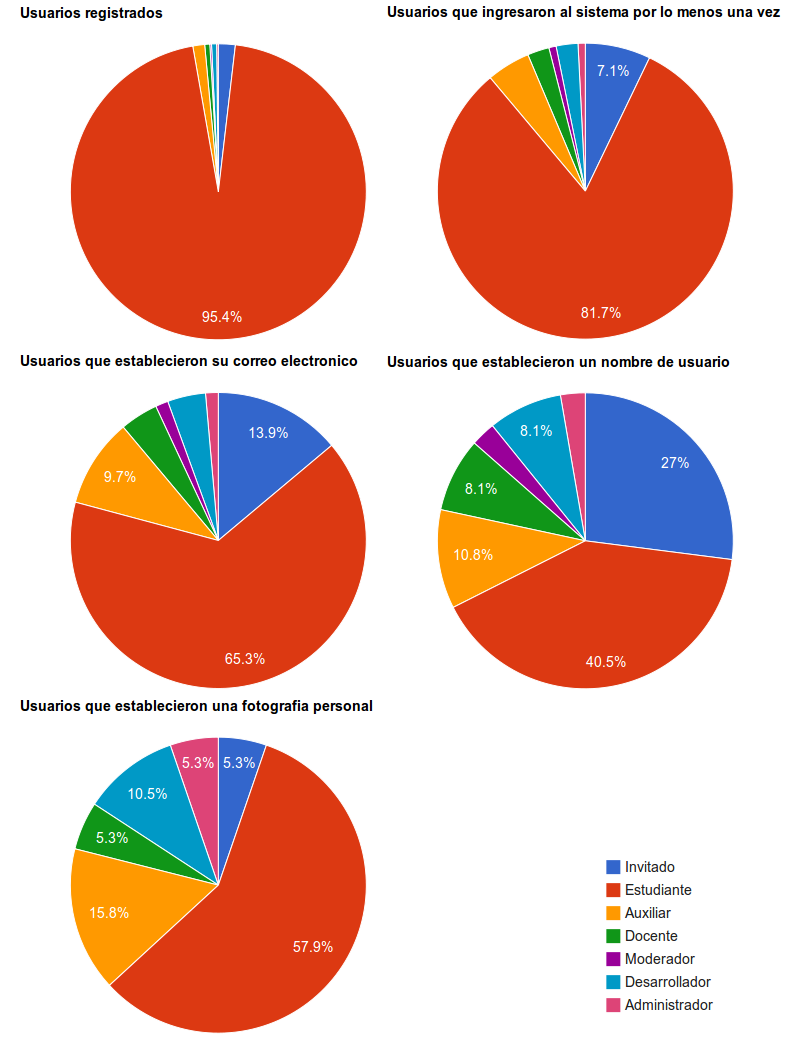
\includegraphics[scale=0.4]{graphics/usuarios_pie_1.png}
%\caption {Porcentajes de intención de los usuarios clasificados por rol}
%\label{usuarios_pie_1}
%\end{figure}

%\begin{figure}[H]
%\centering
%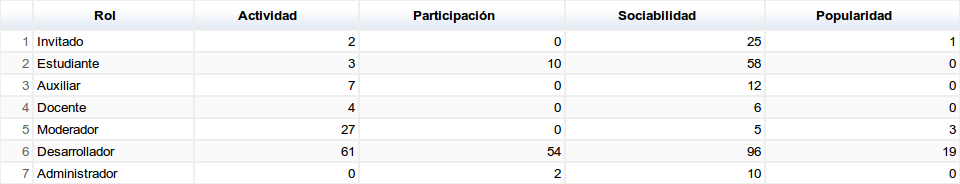
\includegraphics[scale=0.4]{graphics/usuarios_tabla_2.png}
%\caption {Actividad de los usuarios clasificados por rol}
%\label {usuarios_tabla_2}
%\end{figure}

%\begin{figure}[H]
%\centering
%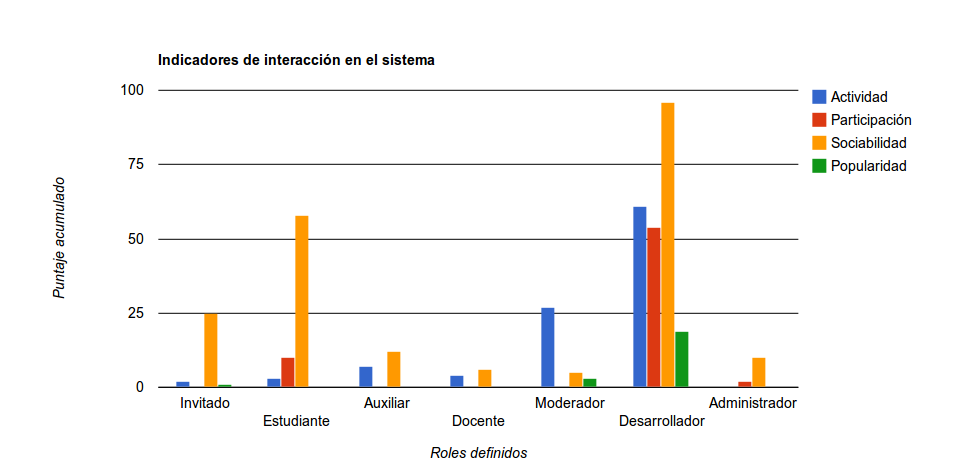
\includegraphics[scale=0.4]{graphics/usuarios_bars_2.png}
%\caption {Diagrama de barras de la actividad de los usuarios clasificados por
%rol}
%\label {usuarios_bars_2}
%\end{figure}

%\begin{figure}[H]
%\centering
%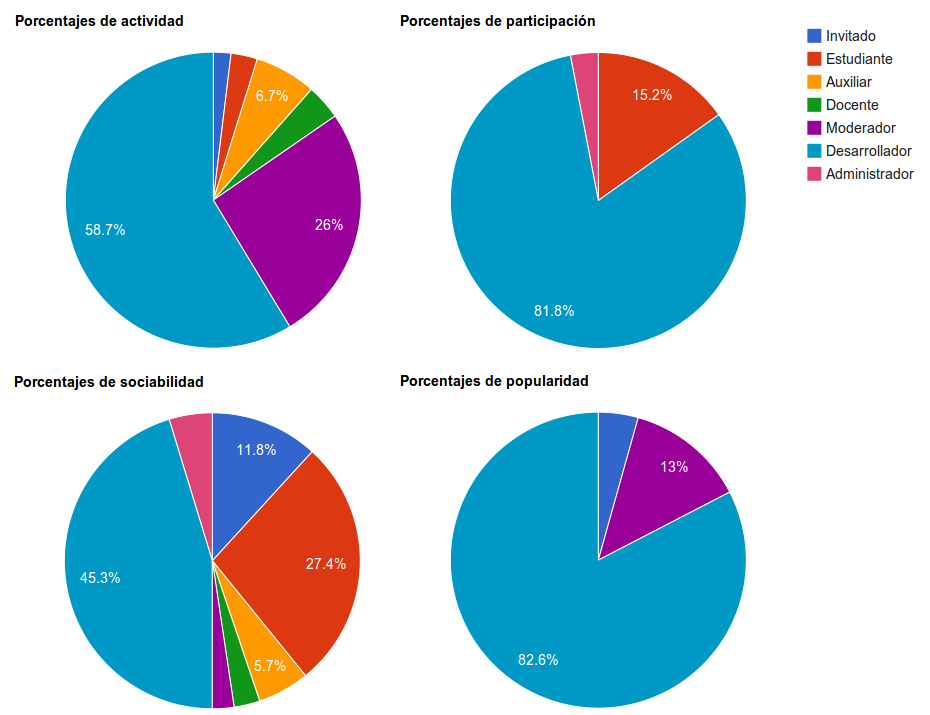
\includegraphics[scale=0.4]{graphics/usuarios_pie_2.png}
%\caption {Porcentajes de actividad clasificados por rol}
%\label {usuarios_pie_2}
%\end{figure}

\subsection{Contactos}

%Considerando los indicadores de sociabilidad, puede apreciarse la matriz de
%adyacencias (Figura \ref{contactos_matriz}) de la red social, puede verse que
%los enlaces fuertes son casi exclusividad propia de los desarrolladores, siendo
%entre los otros roles predominantes los enlaces débiles. Puede verse también
%una sutil relación entre los usuarios que establecieron el nombre de usuario en
%su perfil, y los niveles de sociabilidad. Cuya interrelación, es motivo de
%seguimiento e intención de demostración.

%\begin{figure}[H]
%\centering
%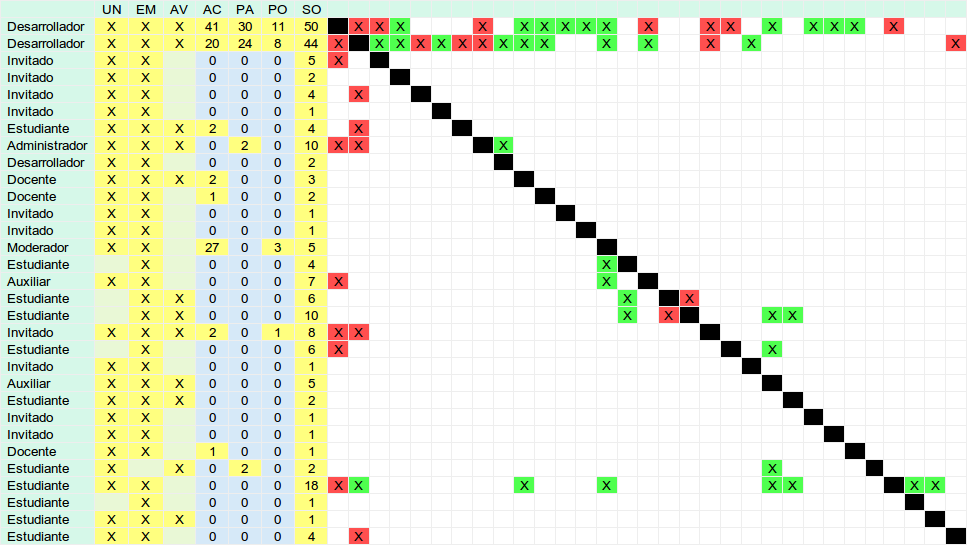
\includegraphics[scale=0.4]{graphics/contactos_matriz.png}
%\caption {Matriz de adyacencia de la red social}
%\label {contactos_matriz}
%\end{figure}

\subsection{Espacios Virtuales}

%En la Figura \ref{espacios_tabla_1} pueden verse los distintos tipos de
%espacios virtuales y sus indicadores propios, entre los que destaca la
%supremacía del espacio portada, por sobre cualquier otro espacio, siendo el que 
%capta mas audiencia de entre los espacios. También es notorio el ausente uso de
%espacios para equipos de trabajo en los grupos, cosa que puede ser debida a las
%escasez de grupos registrados. Si bien la portada acapara la mayor audiencia,
%no acapara la mayor cantidad de recursos (Figura \ref{espacios_bars_1}),
%llevándose los espacios de comunidades un 45\% del contenido del sitio, 
%reforzando la teoría de fomento hacia los espacios menos formales (Figura
%\ref{espacios_pie_1}).

%\begin{figure}[H]
%\centering
%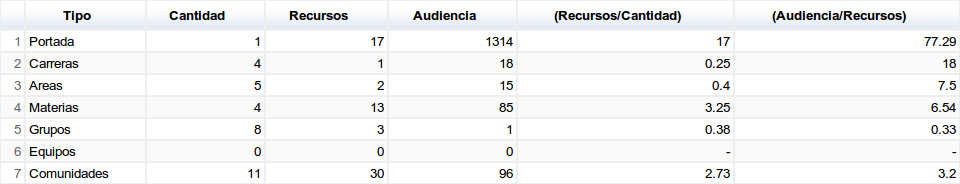
\includegraphics[scale=0.4]{graphics/espacios_tabla_1.png}
%\caption {Clasificación de los espacios y su actividad}
%\label {espacios_tabla_1}
%\end{figure}

%\begin{figure}[H]
%\centering
%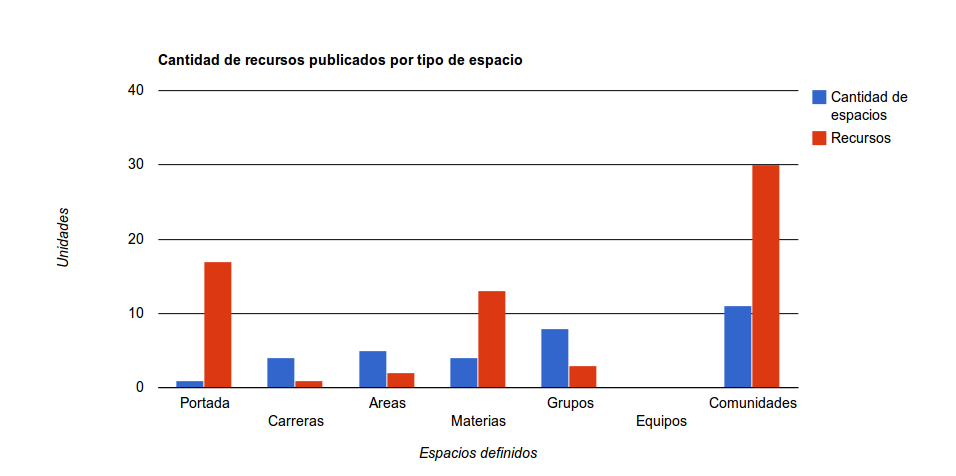
\includegraphics[scale=0.4]{graphics/espacios_bars_1.png}
%\caption {Diagrama de barras de los espacios y sus recursos}
%\label {espacios_bars_1}
%\end{figure}

%\begin{figure}[H]
%\centering
%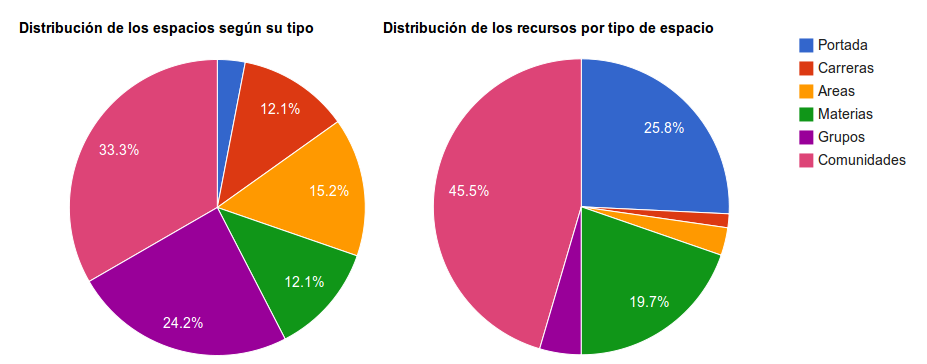
\includegraphics[scale=0.4]{graphics/espacios_pie_1.png}
%\caption {Porcentajes de los espacios y sus recursos seg\'un su tipo}
%\label {espacios_pie_1}
%\end{figure}

\subsection{Recursos}

%Los recursos pueden ser de varios tipos (Figura \ref{recursos_tabla_1}),
%destacando la gran cantidad de notas (Figura \ref{recursos_bars_1}) por sobre
%los otros tipos de recursos, pudiendo esto deberse a la inmensa facilidad de
%creación de estas. Aun así son las fotografías la que en proporción reciben
%mejor audiencia, y son los archivos los que reciben mayor cantidad de 
%comentarios (Figura \ref{recursos_pie_1}).

%\begin{figure}[H]
%\centering
%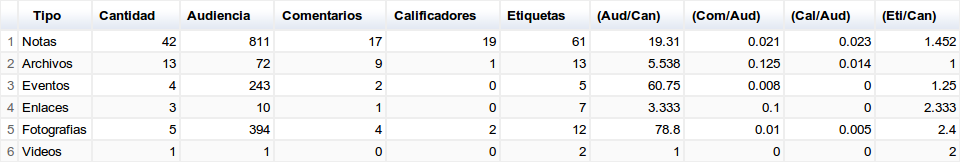
\includegraphics[scale=0.4]{graphics/recursos_tabla_1.png}
%\caption {Clasificación de los recursos según su tipo}
%\label {recursos_tabla_1}
%\end{figure}

%\begin{figure}[H]
%\centering
%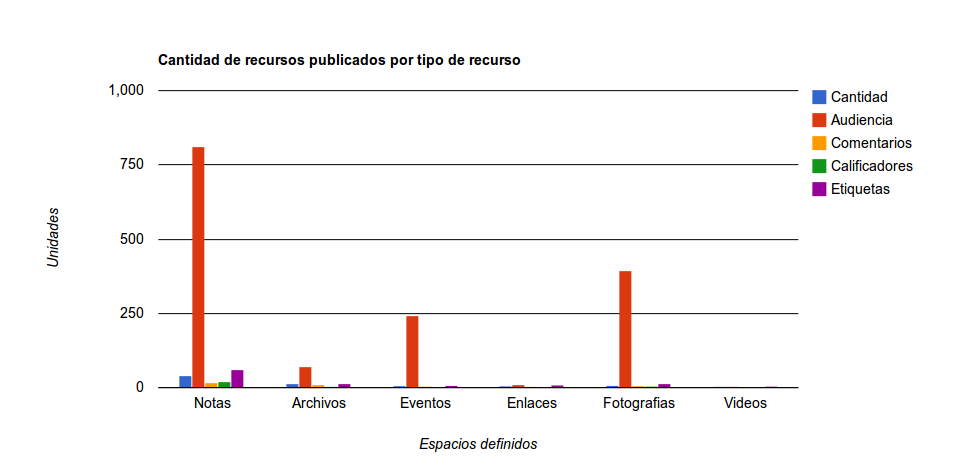
\includegraphics[scale=0.4]{graphics/recursos_bars_1.png}
%\caption {Diagrama de barras de los recursos y sus niveles de repercusión}
%\label {recursos_bars_1}
%\end{figure}

%\begin{figure}[H]
%\centering
%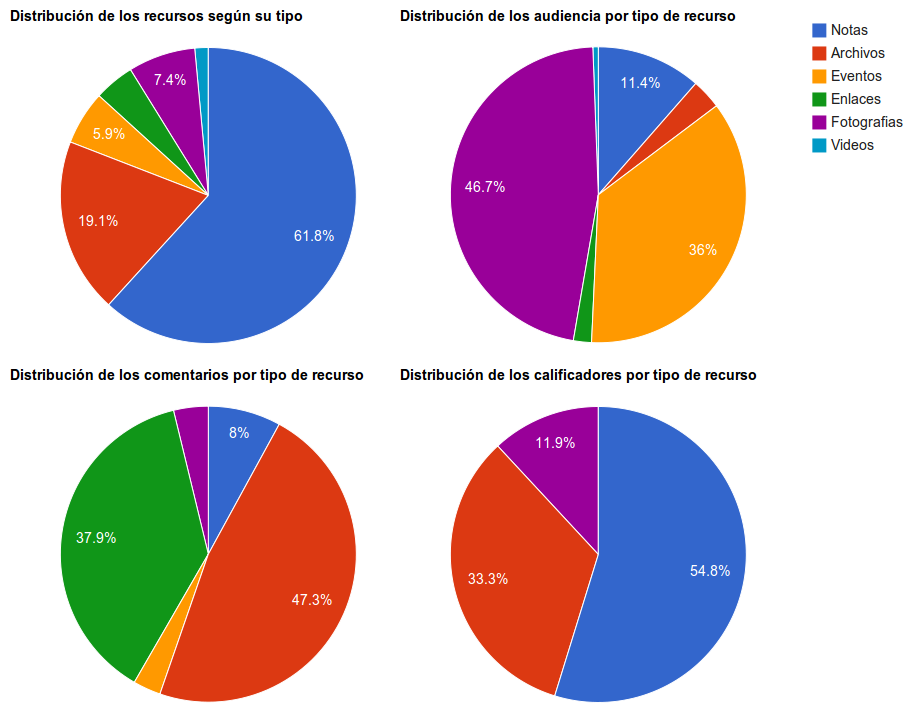
\includegraphics[scale=0.4]{graphics/recursos_pie_1.png}
%\caption {Porcentajes de los recursos según su tipo}
%\label {recursos_pie_1}
%\end{figure}

\subsection{Linea de tiempo}

%Finalizados los elementos propios de la herramienta, se observan ahora las
%lineas de tiempo, donde se presentan los tiempos en los que estos elementos han
%sido creados.
%En la Figura \ref{tiempos_area_1} puede apreciarse en la linea de creación de
%los usuarios, los registros automáticos de los estudiantes, de parte del
%docente de su materia, siendo la creación de usuarios la linea predominante en
%esta gráfica.

%\begin{figure}[H]
%\centering
%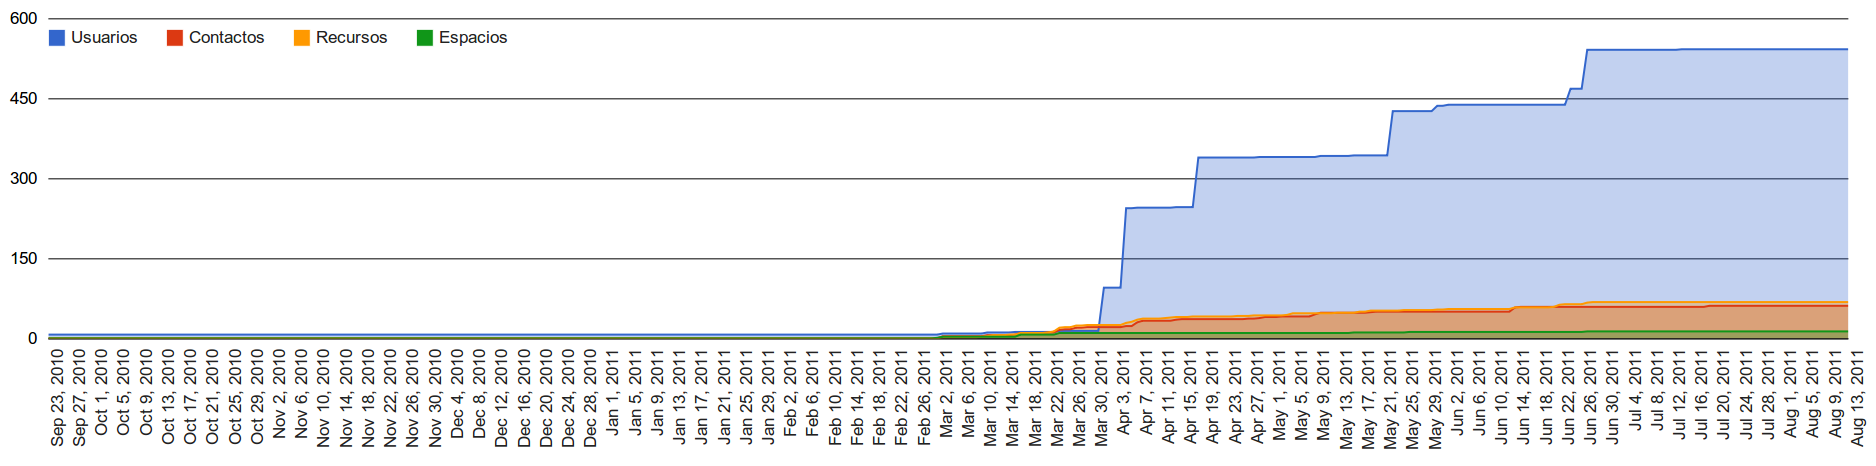
\includegraphics[scale=0.25]{graphics/tiempos_area_1.png}
%\caption {Linea de tiempo de la creación de elementos en el sistema}
%\label {tiempos_area_1}
%\end{figure}

%En la Figura \ref{tiempos_area_2} resalta la curiosa relación entre las lineas
%de creación de recursos y la de creación de contactos, siendo esta la linea que
%determina todo el objeto de investigación.

%\begin{figure}[H]
%\centering
%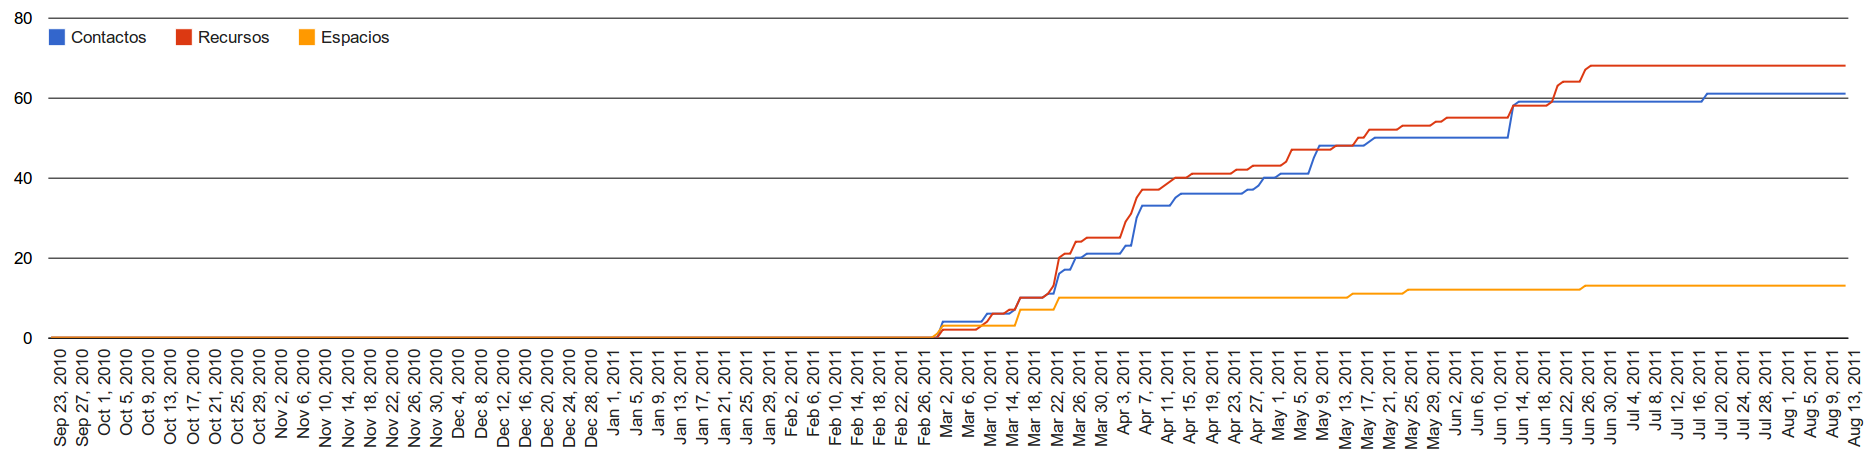
\includegraphics[scale=0.25]{graphics/tiempos_area_2.png}
%\caption {Linea de tiempo de la creación de elementos en el sistema}
%\label {tiempos_area_2}
%\end{figure}

\section{Conclusiones}
\section{Recomendaciones}
